\textbf{\hypertarget{P7}{[\,Suggested Time: 20 mins \textbar \, Total Marks: 10 \textbar \, Challenging\,]}} \\\\
\textbf{Fermat's Principle of Least Time} \\
\textit{Fermat's Principle of Least Time states that out of all neighbouring paths available, \\
        light travels between two points along the path that requires the least time.\\
        \\
        Consider a light ray from a source which strikes a mirror and is reflected. Let A be \\
        a point on the ray before it strikes the mirror and B be the point on the ray after \\
        reflection. v m/s  is the speed of light. \\
        \\
        A coordinate system is placed in a plane such that the x-axis runs along the mirror's \\
        surface and the point A lies on the y-axis.
        \\
}
\begin{center}
    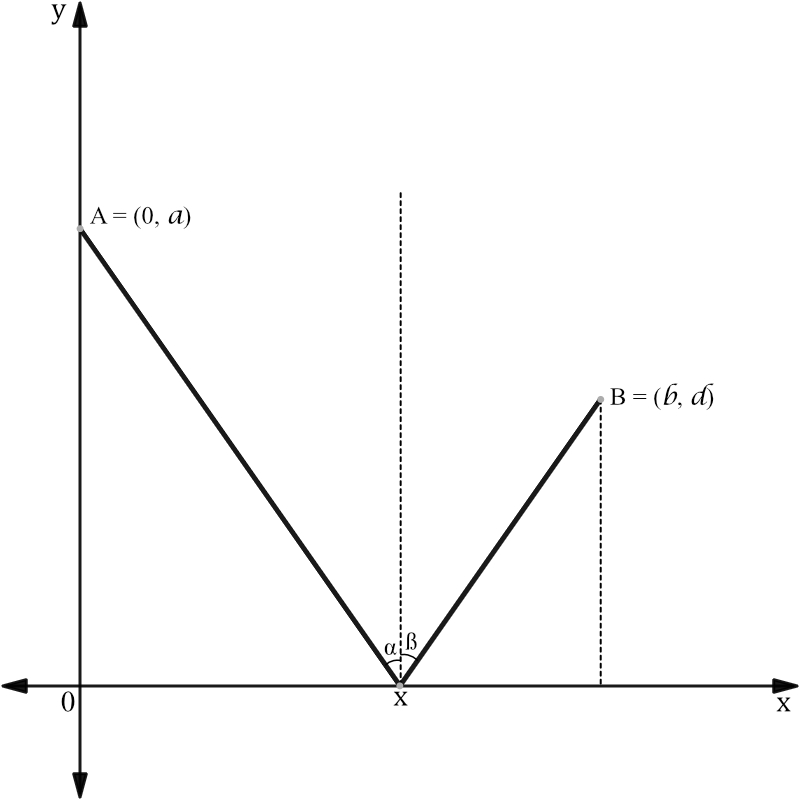
\includegraphics[scale=0.4]{Problem 7 - Reference Diagram.jpg}
\end{center}

\newpage

\textit{Prove that the angle of incidence \(\alpha\) is equal to the angle of reflection \(\beta\). \\
        (Proof that T is minimum is not required)} \qnmark{10}

%%%%%%%%%%%%%%%%%%
%%%%%Solution%%%%%
%%%%%%%%%%%%%%%%%%

%\begin{comment}
    \textit{\\ Note that \(\displaystyle \tan{\alpha} = \frac{x}{a}\) and \(\displaystyle \tan{\beta} = \frac{b-x}{d}\)}

    %%%%%Finding the function T%%%%%
    \begin{align*}
        \displaystyle T &= \frac{Distance}{Speed} \\
        \displaystyle   &= \frac{|Ax|}{v}+\frac{|Bx|}{v} \onemark \\
        \displaystyle   &= \frac{1}{v}\sqrt{a^{2}+x^{2}} + \frac{1}{v}\sqrt{d^{2}+(b-x)^{2}} \onemark \\
        \displaystyle   &= \frac{1}{v}\left(\sqrt{a^{2}+x^{2}}+\sqrt{d^{2}+(b-x)^{2}}\right)
    \end{align*}
    
    %%%%%Differentiating T w.r.t. x%%%%%
    \begin{align*}
        \displaystyle \therefore \frac{dT}{dx} &= \frac{1}{v}\left(\frac{x}{\sqrt{a^{2}+x^{2}}}-\frac{b-x}{\sqrt{d^{2}+(b-x)^2}}\right) \twomark \\
        \displaystyle                          &= \left(\frac{x\sqrt{d^{2}+(b-x)^2}-(b-x)\sqrt{a^{2}+x^{2}}}{v\sqrt{\left(a^{2}+x^{2}\right)\left(d^{2}+(b-x)^{2}\right)}}\right) \onemark \\
    \end{align*}

    %%%%%Finding the min. value of T%%%%%
    \textit{For minimum T,}
    \begin{align*}
        \displaystyle \frac{dT}{dx} &= 0 \\
        \displaystyle \frac{x\sqrt{d^{2}+(b-x)^2}-(b-x)\sqrt{a^{2}+x^{2}}}{v\sqrt{\left(a^{2}+x^{2}\right)\left(d^{2}+(b-x)^{2}\right)}} &= 0 \onemark \\
        \displaystyle                                                                      x\sqrt{d^{2}+(b-x)^2}-(b-x)\sqrt{a^{2}+x^{2}} &= 0 \onemark \\
        \displaystyle                                                                                              x\sqrt{d^{2}+(b-x)^2} &= (b-x)\sqrt{a^{2}+x^{2}} \\
        \displaystyle                                                                                    x^{2}\left(d^{2}+(b-x)^2\right) &= (b-x)^{2}\left(a^{2}+x^{2}\right) \onemark \\
        \displaystyle                                                            x^{2}d^{2}+x^{2}(b-x)^{2}-a^{2}(b-x)^{2}-x^{2}(b-x)^{2} &= 0 \\
        \displaystyle                                                                                          x^{2}d^{2}-a^{2}(b-x)^{2} &= 0 \\
        \displaystyle                                                                                                         x^{2}d^{2} &= a^{2}(b-x)^{2} \\
        \displaystyle                                                                                                                 xd &= a(b-x) \\
        \displaystyle                                                                                                        \frac{x}{a} &= \frac{b-x}{d} \\
        \displaystyle                                                                                                       \tan{\alpha} &= \tan{\beta} \onemark
    \end{align*}
    \begin{gather*}
        Since \; both \; \alpha \;\&\; \beta \; are \; acute, \\
        \implies \alpha = \beta \tag*{\qedsymbol} \\ \onemark
    \end{gather*}

%\end{comment}

\newpage \ \newpage